\documentclass[a4paper,11pt,oneside]{book}

% packages 
\usepackage{arsclassica}    % fancy layout
\usepackage[english]{babel}\addto{\captionsenglish}{\renewcommand{\bibname}{References}}
\usepackage{caption}         % figure captions
\usepackage[square,numbers,super,sort&compress]{natbib}  % bibliography style
\usepackage[cc]{titlepic}    % enable logo on title page
\usepackage{graphicx}       % logo related
\usepackage{pdfpages}

\usepackage{standalone}
\standalonetrue

% GO term margins 
\usepackage{longtable}
\usepackage{geometry}

% bibliography
\bibliographystyle{../thesis}

% don't hang captions
\captionsetup{format=plain}

\graphicspath {{../figs/}}

% title setup
\title{ \vspace{3in} Unravelling higher order genome organisation {\small [working
    title]} \\ \vspace{2em} {\large {\bf Results 5: Collaborations}} }
\author{Benjamin L. Moore}
\titlepic{\vspace{2.2in} 
\includegraphics[width=\textwidth]{/Users/benmoore/hvl/1yrReport/figs/igmm.png}}

\begin{document}


\chapter{Appendices}

% GO term tables
\setcounter{table}{0}
\makeatletter 
\renewcommand{\thetable}{A\@arabic\c@table}
\makeatother

\newgeometry{left=2cm,right=2cm}

{\tiny 
\begin{longtable}{lllllll}
\caption[Gm12878 functional enrichments in regions of variable structure.]{
{\bf 
Gm12878 functional enrichments in regions of variable structure.
} FE: fold enrichment; FDR: false discovery rate.
}\label{tab:gmgo}\\
\endfirsthead
Category          & Term                                          &
Count & \%   & FE & $p$-value   & FDR      \\
GOTERM\_CC\_FAT   & GO:0005882~intermediate filament              & 36    & 4.20 & 4.90            & 6.42E-15 & 8.95E-12 \\
GOTERM\_CC\_FAT   & GO:0045111~intermediate filament cytoskeleton & 36    & 4.20 & 4.79            & 1.35E-14 & 1.87E-11 \\
SP\_PIR\_KEYWORDS & keratin                                       & 31    & 3.62 & 5.64            & 1.72E-14 & 2.47E-11 \\
INTERPRO          & IPR007951:PMG                                 & 11    & 1.28 & 25.11           & 9.80E-14 & 1.56E-10
\end{longtable}
}

\clearpage

{\scriptsize 
\begin{longtable}{lllllll}
\caption[H1 hESC functional enrichments in regions of variable structure.]{ {\bf
H1 hESC functional enrichments in regions of variable structure. }
FE: fold enrichment; FDR: false discovery rate.
}\label{tab:h1go}\\
\endfirsthead

Category          & Term
& Count & \%    & FE & $p$-value   & FDR      \\
PIR\_SUPERFAMILY  & PIRSF003152:G protein-coupled olfactory receptor, class II      & 116   & 10.55 & 6.64            & 3.25E-68 & 4.41E-65 \\
INTERPRO          & IPR000725:Olfactory receptor                                    & 116   & 10.55 & 6.53            & 7.58E-63 & 1.21E-59 \\
SP\_PIR\_KEYWORDS & olfaction                                                       & 116   & 10.55 & 6.40            & 2.07E-61 & 2.97E-58 \\
GOTERM\_MF\_FAT   & GO:0004984~olfactory receptor activity                          & 116   & 10.55 & 6.13            & 1.30E-60 & 1.97E-57 \\
GOTERM\_BP\_FAT   & GO:0007608~sensory perception of smell                          & 117   & 10.64 & 5.96            & 1.91E-59 & 3.35E-56 \\
GOTERM\_BP\_FAT   & GO:0007606~sensory perception of chemical stimulus              & 118   & 10.73 & 5.37            & 1.71E-54 & 3.01E-51 \\
KEGG\_PATHWAY     & hsa04740:Olfactory transduction                                 & 108   & 9.82  & 4.94            & 8.72E-51 & 1.03E-47 \\
SP\_PIR\_KEYWORDS & sensory transduction                                            & 125   & 11.36 & 4.58            & 2.61E-48 & 3.74E-45 \\
INTERPRO          & IPR017452:GPCR, rhodopsin-like superfamily                      & 131   & 11.91 & 4.03            & 1.40E-44 & 2.24E-41 \\
INTERPRO          & IPR000276:7TM GPCR, rhodopsin-like                              & 131   & 11.91 & 4.02            & 1.68E-44 & 2.68E-41 \\
PIR\_SUPERFAMILY  & PIRSF800006:rhodopsin-like G protein-coupled receptors          & 131   & 11.91 & 3.63            & 5.04E-43 & 6.85E-40 \\
GOTERM\_BP\_FAT   & GO:0007600~sensory perception                                   & 138   & 12.55 & 3.54            & 4.78E-41 & 8.40E-38 \\
SP\_PIR\_KEYWORDS & g-protein coupled receptor                                      & 136   & 12.36 & 3.62            & 1.69E-40 & 2.42E-37 \\
GOTERM\_BP\_FAT   & GO:0050890~cognition                                            & 143   & 13.00 & 3.23            & 5.34E-38 & 9.38E-35 \\
SP\_PIR\_KEYWORDS & transducer                                                      & 137   & 12.45 & 3.39            & 1.48E-37 & 2.12E-34 \\
GOTERM\_BP\_FAT   & GO:0050877~neurological system process                          & 163   & 14.82 & 2.72            & 3.85E-34 & 6.76E-31 \\
GOTERM\_BP\_FAT   & GO:0007186~G-protein coupled receptor protein signaling pathway & 148   & 13.45 & 2.77            & 1.36E-31 & 2.40E-28 \\
SP\_PIR\_KEYWORDS & receptor                                                        & 172   & 15.64 & 2.31            & 3.72E-26 & 5.33E-23 \\
GOTERM\_BP\_FAT   & GO:0007166~cell surface receptor linked signal transduction     & 188   & 17.09 & 2.06            & 8.02E-24 & 1.41E-20 \\
SP\_PIR\_KEYWORDS & cell membrane                                                   & 198   & 18.00 & 1.86            & 5.96E-19 & 8.52E-16 \\
UP\_SEQ\_FEATURE  & topological domain:Extracellular                                & 227   & 20.64 & 1.72            & 1.26E-17 & 2.20E-14 \\
UP\_SEQ\_FEATURE  & topological domain:Cytoplasmic                                  & 250   & 22.73 & 1.52            & 1.13E-12 & 1.98E-09 \\
UP\_SEQ\_FEATURE  & disulfide bond                                                  & 211   & 19.18 & 1.56            & 9.11E-12 & 1.60E-08 \\
SP\_PIR\_KEYWORDS & disulfide bond                                                  & 214   & 19.45 & 1.52            & 6.20E-11 & 8.88E-08 \\
UP\_SEQ\_FEATURE  & glycosylation site:N-linked (GlcNAc...)                         & 285   & 25.91 & 1.41            & 7.31E-11 & 1.28E-07 \\
GOTERM\_CC\_FAT   & GO:0005886~plasma membrane                                      & 255   & 23.18 & 1.37            & 1.26E-09 & 1.77E-06 \\
SP\_PIR\_KEYWORDS & glycoprotein                                                    & 289   & 26.27 & 1.37            & 1.83E-09 & 2.61E-06 \\
GOTERM\_CC\_FAT   & GO:0016021~integral to membrane                                 & 328   & 29.82 & 1.27            & 9.34E-09 & 1.31E-05 \\
SP\_PIR\_KEYWORDS & transmembrane                                                   & 317   & 28.82 & 1.31            & 1.37E-08 & 1.96E-05 \\
UP\_SEQ\_FEATURE  & transmembrane region                                            & 314   & 28.55 & 1.31            & 2.03E-08 & 3.56E-05 \\
GOTERM\_CC\_FAT   & GO:0031224~intrinsic to membrane                                & 333   & 30.27 & 1.24            & 7.49E-08 & 1.05E-04 \\
SMART             & SM00355:ZnF\_C2H2                                               & 69    & 6.27  & 1.86            & 4.23E-07 & 5.43E-04 \\
UP\_SEQ\_FEATURE  & zinc finger region:C2H2-type 5                                  & 55    & 5.00  & 2.08            & 5.12E-07 & 8.99E-04 \\
UP\_SEQ\_FEATURE  & zinc finger region:C2H2-type 4                                  & 57    & 5.18  & 2.01            & 8.49E-07 & 0.0015   \\
INTERPRO          & IPR013087:Zinc finger, C2H2-type/integrase, DNA-binding         & 59    & 5.36  & 1.94            & 1.73E-06 & 0.0028   \\
UP\_SEQ\_FEATURE  & zinc finger region:C2H2-type 2                                  & 58    & 5.27  & 1.95            & 1.73E-06 & 0.0030   \\
SP\_PIR\_KEYWORDS & membrane                                                        & 372   & 33.82 & 1.21            & 2.69E-06 & 0.0038   \\
INTERPRO          & IPR015880:Zinc finger, C2H2-like                                & 69    & 6.27  & 1.78            & 4.09E-06 & 0.0065   \\
UP\_SEQ\_FEATURE  & zinc finger region:C2H2-type 8                                  & 44    & 4.00  & 2.14            & 4.13E-06 & 0.0073   \\
UP\_SEQ\_FEATURE  & zinc finger region:C2H2-type 3                                  & 58    & 5.27  & 1.90            & 4.43E-06 & 0.0078   \\
UP\_SEQ\_FEATURE  & zinc finger region:C2H2-type 7                                  & 46    & 4.18  & 2.06            & 5.87E-06 & 0.0103   \\
INTERPRO          & IPR007087:Zinc finger, C2H2-type                                & 67    & 6.09  & 1.75            & 9.19E-06 & 0.0147   \\
UP\_SEQ\_FEATURE  & zinc finger region:C2H2-type 6                                  & 48    & 4.36  & 1.99            & 9.83E-06 & 0.0173  
\end{longtable}
}

\clearpage

{\scriptsize 
\begin{longtable}{lllllll}
\caption[K562 functional enrichments in regions of variable structure.]{
{\bf K562 functional enrichments in regions of variable structure. }
FE: fold enrichment; FDR: false discovery rate.
}\label{tab:k5go}\\
\endfirsthead

%\begin{tabular}
Category          & Term
& Count & \%    & FE & $p$-value   & FDR      \\
PIR\_SUPERFAMILY  & PIRSF038651:G protein-coupled olfactory receptor, class I       & 26    & 7.08  & 24.94           & 7.86E-30 & 8.99E-27 \\
GOTERM\_MF\_FAT   & GO:0004984~olfactory receptor activity                          & 40    & 10.90 & 6.12            & 7.39E-20 & 1.01E-16 \\
INTERPRO          & IPR000725:Olfactory receptor                                    & 39    & 10.63 & 6.18            & 3.00E-19 & 4.29E-16 \\
SP\_PIR\_KEYWORDS & olfaction                                                       & 39    & 10.63 & 6.15            & 4.55E-19 & 6.09E-16 \\
GOTERM\_BP\_FAT   & GO:0007608~sensory perception of smell                          & 39    & 10.63 & 5.48            & 1.19E-17 & 1.94E-14 \\
SP\_PIR\_KEYWORDS & sensory transduction                                            & 44    & 11.99 & 4.60            & 8.72E-17 & 1.44E-13 \\
GOTERM\_BP\_FAT   & GO:0007606~sensory perception of chemical stimulus              & 39    & 10.63 & 4.89            & 6.32E-16 & 1.09E-12 \\
KEGG\_PATHWAY     & hsa04740:Olfactory transduction                                 & 38    & 10.35 & 4.58            & 6.87E-16 & 7.22E-13 \\
INTERPRO          & IPR017452:GPCR, rhodopsin-like superfamily                      & 43    & 11.72 & 3.72            & 2.96E-13 & 4.23E-10 \\
INTERPRO          & IPR000276:7TM GPCR, rhodopsin-like                              & 43    & 11.72 & 3.72            & 3.10E-13 & 4.43E-10 \\
SP\_PIR\_KEYWORDS & transducer                                                      & 46    & 12.53 & 3.26            & 4.97E-12 & 6.65E-09 \\
SP\_PIR\_KEYWORDS & g-protein coupled receptor                                      & 44    & 11.99 & 3.35            & 6.34E-12 & 8.48E-09 \\
PIR\_SUPERFAMILY  & PIRSF800006:rhodopsin-like G protein-coupled receptors          & 42    & 11.44 & 3.26            & 6.34E-12 & 7.26E-09 \\
GOTERM\_BP\_FAT   & GO:0007600~sensory perception                                   & 45    & 12.26 & 3.18            & 1.10E-11 & 1.80E-08 \\
GOTERM\_BP\_FAT   & GO:0050890~cognition                                            & 46    & 12.53 & 2.87            & 1.87E-10 & 3.07E-07 \\
UP\_SEQ\_FEATURE  & zinc finger region:C2H2-type 10                                 & 27    & 7.36  & 4.64            & 1.94E-10 & 3.10E-07 \\
UP\_SEQ\_FEATURE  & zinc finger region:C2H2-type 1; degenerate                      & 17    & 4.63  & 8.23            & 2.35E-10 & 3.77E-07 \\
GOTERM\_BP\_FAT   & GO:0007186~G-protein coupled receptor protein signaling pathway & 51    & 13.90 & 2.63            & 2.87E-10 & 4.70E-07 \\
UP\_SEQ\_FEATURE  & zinc finger region:C2H2-type 11                                 & 25    & 6.81  & 4.91            & 3.32E-10 & 5.31E-07 \\
UP\_SEQ\_FEATURE  & zinc finger region:C2H2-type 9                                  & 28    & 7.63  & 4.30            & 4.58E-10 & 7.33E-07 \\
UP\_SEQ\_FEATURE  & zinc finger region:C2H2-type 12                                 & 23    & 6.27  & 5.27            & 5.15E-10 & 8.24E-07 \\
SMART             & SM00349:KRAB                                                    & 26    & 7.08  & 4.36            & 7.67E-10 & 8.65E-07 \\
UP\_SEQ\_FEATURE  & zinc finger region:C2H2-type 15                                 & 17    & 4.63  & 7.40            & 1.17E-09 & 1.88E-06 \\
UP\_SEQ\_FEATURE  & zinc finger region:C2H2-type 7                                  & 30    & 8.17  & 3.84            & 1.33E-09 & 2.13E-06 \\
INTERPRO          & IPR001909:Krueppel-associated  box                              & 26    & 7.08  & 4.20            & 3.15E-09 & 4.49E-06 \\
UP\_SEQ\_FEATURE  & domain:KRAB                                                     & 25    & 6.81  & 4.37            & 3.38E-09 & 5.41E-06 \\
UP\_SEQ\_FEATURE  & zinc finger region:C2H2-type 14                                 & 17    & 4.63  & 6.32            & 1.19E-08 & 1.90E-05 \\
UP\_SEQ\_FEATURE  & zinc finger region:C2H2-type 13                                 & 19    & 5.18  & 5.50            & 1.19E-08 & 1.91E-05 \\
UP\_SEQ\_FEATURE  & zinc finger region:C2H2-type 8                                  & 27    & 7.36  & 3.73            & 1.86E-08 & 2.98E-05 \\
UP\_SEQ\_FEATURE  & zinc finger region:C2H2-type 6                                  & 29    & 7.90  & 3.42            & 3.22E-08 & 5.15E-05 \\
INTERPRO          & IPR001089:Small chemokine, C-X-C                                & 7     & 1.91  & 29.85           & 4.94E-08 & 7.06E-05 \\
INTERPRO          & IPR002473:Small chemokine, C-X-C/Interleukin 8                  & 7     & 1.91  & 27.72           & 8.52E-08 & 1.22E-04 \\
GOTERM\_BP\_FAT   & GO:0050877~neurological system process                          & 48    & 13.08 & 2.21            & 2.61E-07 & 4.27E-04 \\
INTERPRO          & IPR018048:Small chemokine, C-X-C, conserved site                & 7     & 1.91  & 22.83           & 3.35E-07 & 4.79E-04 \\
INTERPRO          & IPR002337:Haemoglobin, beta                                     & 5     & 1.36  & 55.44           & 5.04E-07 & 7.20E-04 \\
INTERPRO          & IPR013087:Zinc finger, C2H2-type/integrase, DNA-binding         & 30    & 8.17  & 2.77            & 1.34E-06 & 0.002    \\
SMART             & SM00355:ZnF\_C2H2                                               & 33    & 8.99  & 2.48            & 1.77E-06 & 0.002    \\
SP\_PIR\_KEYWORDS & receptor                                                        & 52    & 14.17 & 2.00            & 2.39E-06 & 0.003    \\
UP\_SEQ\_FEATURE  & zinc finger region:C2H2-type 5                                  & 27    & 7.36  & 2.90            & 2.39E-06 & 0.004    \\
UP\_SEQ\_FEATURE  & zinc finger region:C2H2-type 3                                  & 29    & 7.90  & 2.70            & 3.79E-06 & 0.006    \\
GOTERM\_MF\_FAT   & GO:0047760~butyrate-CoA ligase activity                         & 5     & 1.36  & 38.47           & 3.81E-06 & 0.005    \\
INTERPRO          & IPR007087:Zinc finger, C2H2-type                                & 33    & 8.99  & 2.43            & 5.58E-06 & 0.008    \\
PIR\_SUPERFAMILY  & PIRSF002522:CXC chemokine                                       & 6     & 1.63  & 20.55           & 6.13E-06 & 0.007    \\
SP\_PIR\_KEYWORDS & oxygen carrier                                                  & 5     & 1.36  & 35.19           & 6.39E-06 & 0.009    \\
INTERPRO          & IPR015880:Zinc finger, C2H2-like                                & 33    & 8.99  & 2.39            & 7.71E-06 & 0.011    \\
GOTERM\_BP\_FAT   & GO:0007166~cell surface receptor linked signal transduction     & 59    & 16.08 & 1.78            & 9.41E-06 & 0.015    \\
UP\_SEQ\_FEATURE  & zinc finger region:C2H2-type 16                                 & 11    & 3.00  & 6.18            & 1.14E-05 & 0.018    \\
PIR\_SUPERFAMILY  & PIRSF500045:hemoglobin, vertebrate type                         & 5     & 1.36  & 29.97           & 1.16E-05 & 0.013    \\
UP\_SEQ\_FEATURE  & zinc finger region:C2H2-type 17                                 & 10    & 2.72  & 7.02            & 1.20E-05 & 0.019    \\
UP\_SEQ\_FEATURE  & disulfide bond                                                  & 77    & 20.98 & 1.62            & 1.27E-05 & 0.020    \\
UP\_SEQ\_FEATURE  & topological domain:Extracellular                                & 75    & 20.44 & 1.62            & 1.99E-05 & 0.032    \\
PIR\_SUPERFAMILY  & PIRSF005559:zinc finger protein ZFP-36                          & 13    & 3.54  & 4.58            & 2.22E-05 & 0.025    \\
SP\_PIR\_KEYWORDS & disulfide bond                                                  & 78    & 21.25 & 1.59            & 2.44E-05 & 0.033    \\
UP\_SEQ\_FEATURE  & zinc finger region:C2H2-type 20                                 & 7     & 1.91  & 11.56           & 2.64E-05 & 0.042    \\
SP\_PIR\_KEYWORDS & blood                                                           & 5     & 1.36  & 25.59           & 2.89E-05 & 0.039    \\
SP\_PIR\_KEYWORDS & cell membrane                                                   & 63    & 17.17 & 1.70            & 3.07E-05 & 0.041   
%\end{tabular}

\end{longtable}
}

\restoregeometry

% additional figures

% GO term tables
\setcounter{figure}{0}
\makeatletter 
\renewcommand{\thefigure}{S\@arabic\c@figure}
\makeatother

\begin{figure}
\begin{center}
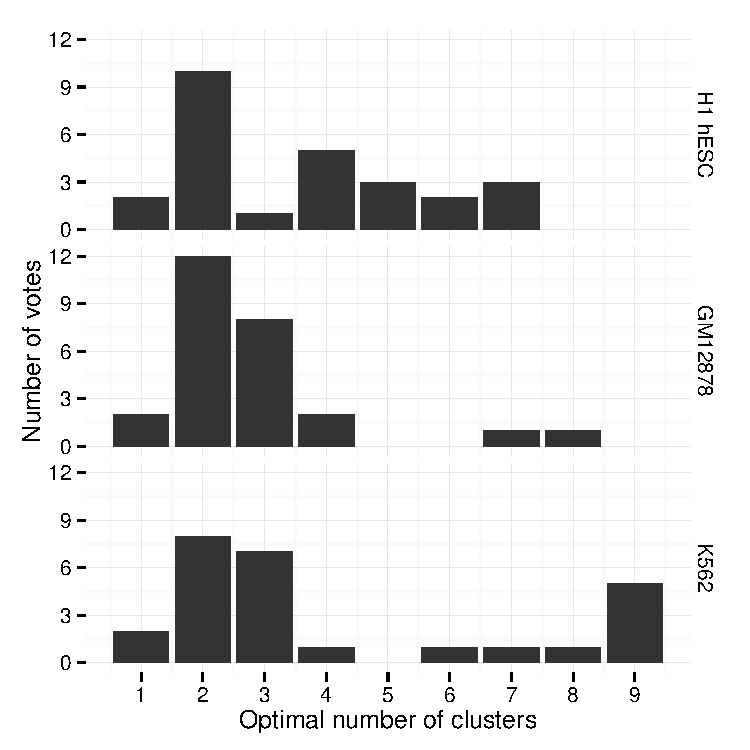
\includegraphics[width=4in]{nbclust.pdf}
\captionsetup{width=\textwidth}
\caption[Optimal $k$ cluster selection by majority vote from multiple algorithms.]{ {\bf Optimal $k$ cluster selection by majority vote from multiple algorithms.}
30 methods for selecting the optimal number of clusters were applied to averaged TAD feature enrichments in each cell type. In each case, the most-selected partition was for two clusters. Performed using the \texttt{NbClust} R package.\cite{Charrad2014}
}\label{fig:nbclust}
\end{center}
\end{figure} 

\begin{figure}
\begin{center}
\makebox[\textwidth][c]{ 
	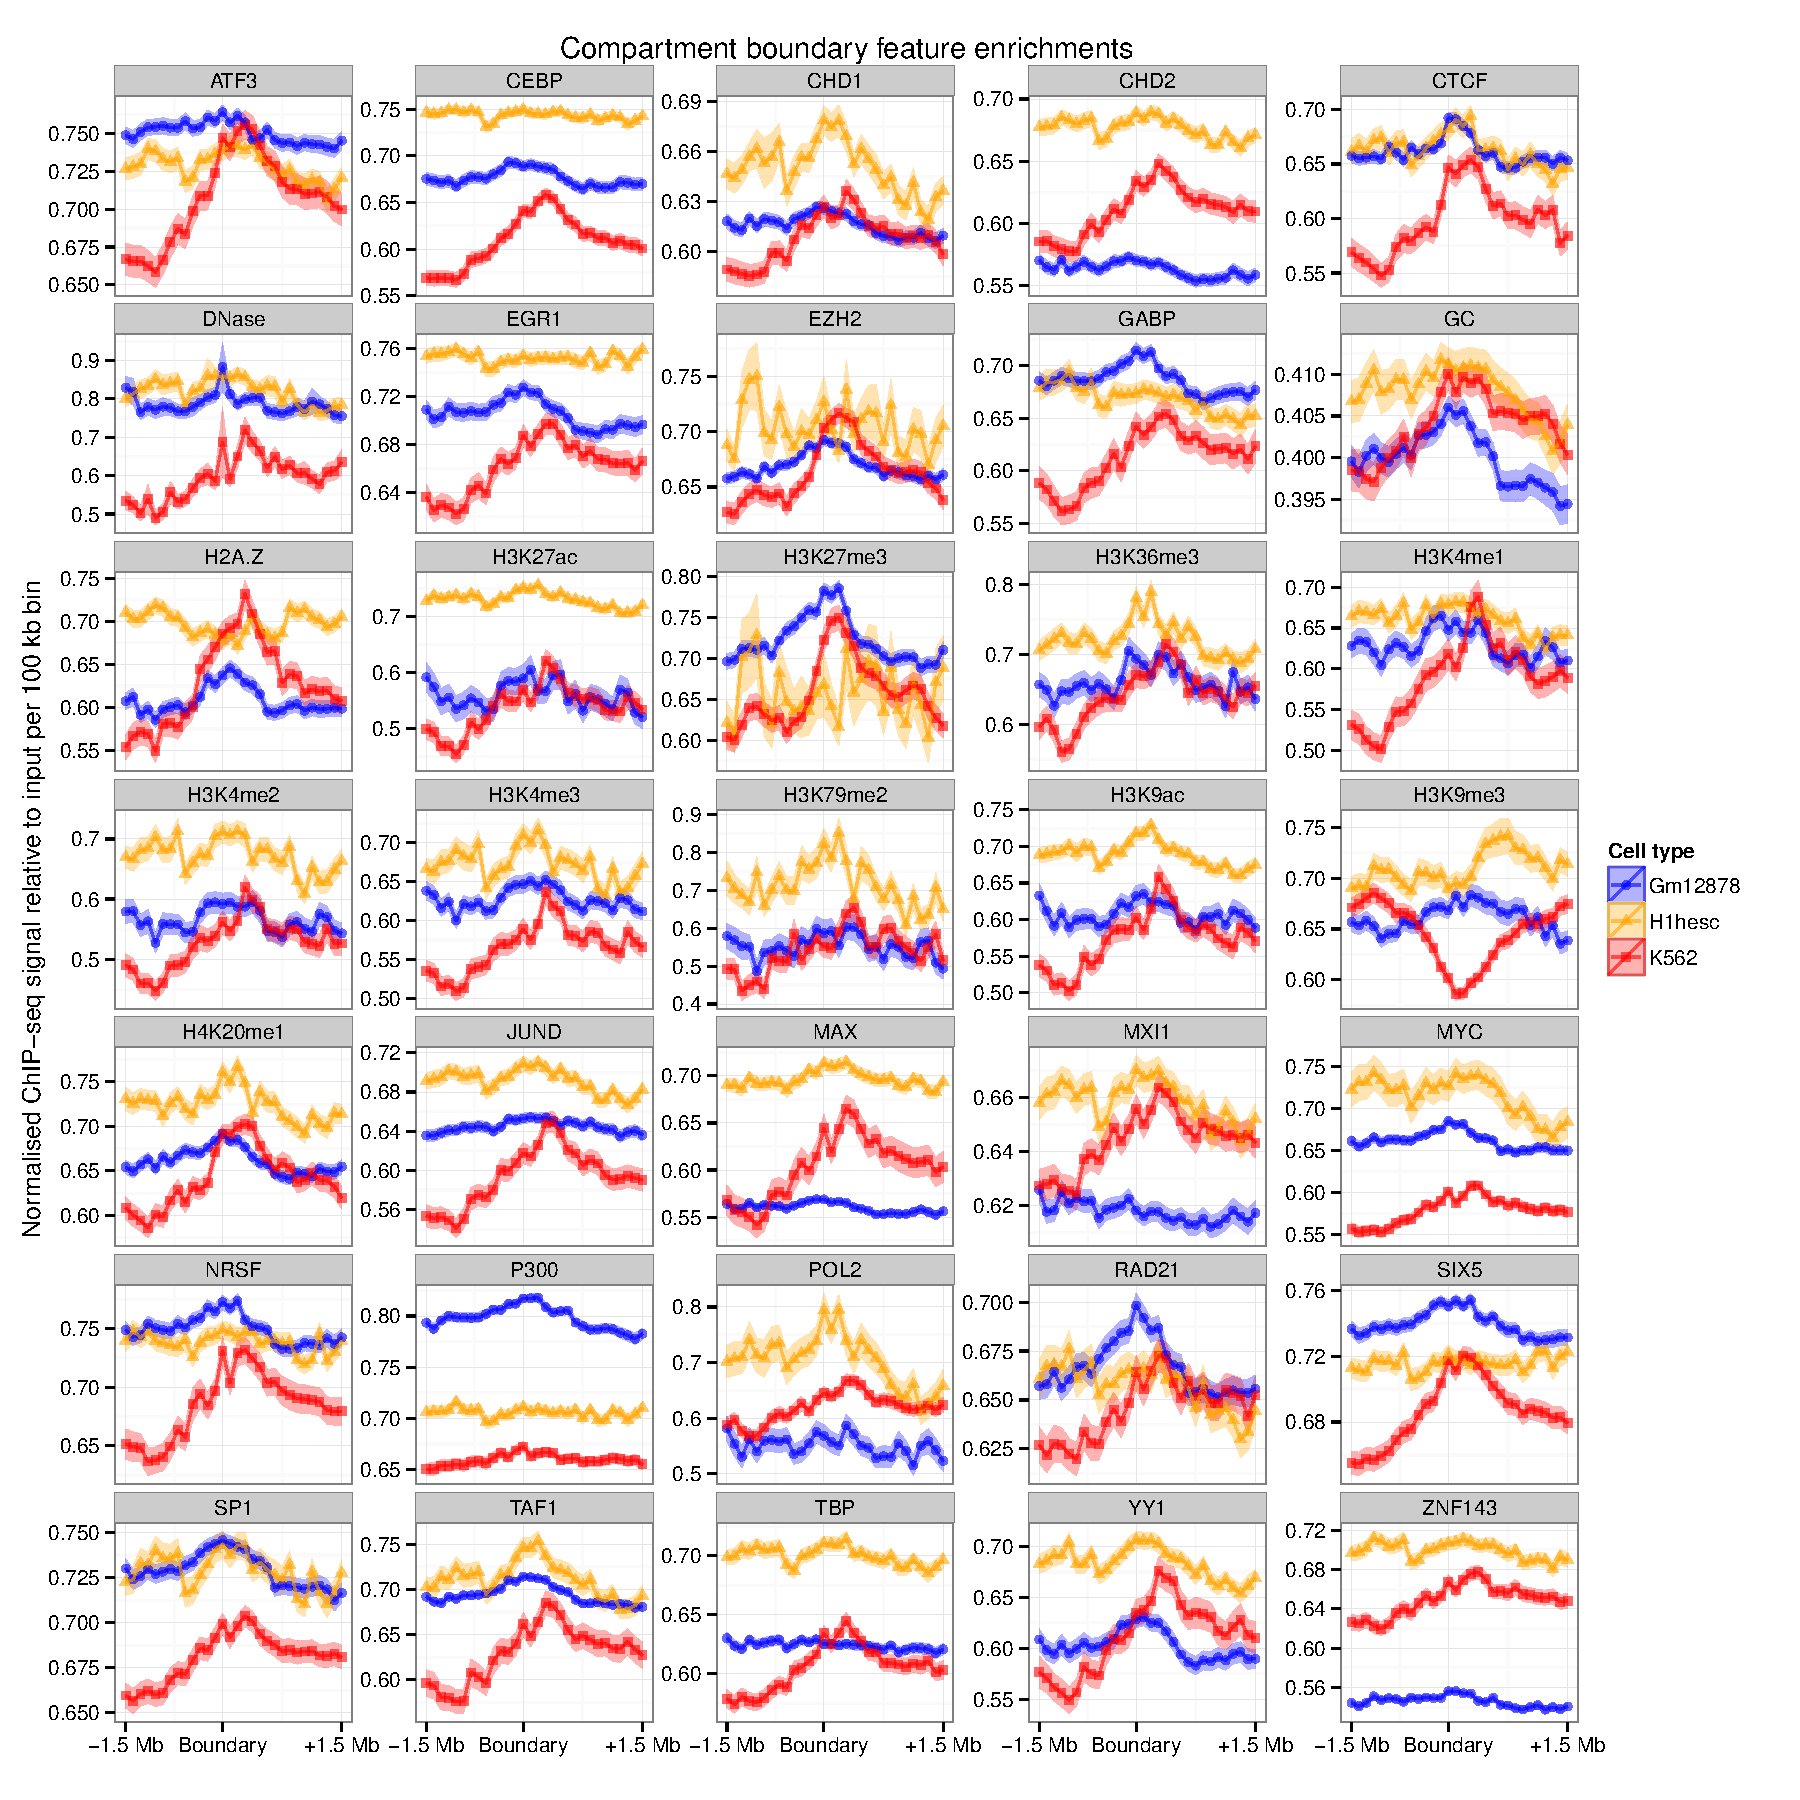
\includegraphics[width=6.8in]{orientatedCbounds.pdf}
}
\captionsetup{width=\textwidth}
\caption[Compartment boundary enrichments and depletions.]{ {\bf Compartment boundary enrichments and depletions.}
35 features were averaged over 3 Mb windows centred on compartment boundaries genome-wide ($30 \times 100$ kb bins). Boundaries are orientated as A to B transitions. Ribbons represent $95\%$ confidence intervals of the mean at each position.
}\label{fig:allcompsorientated}
\end{center}
\end{figure} 

\clearpage

% paper
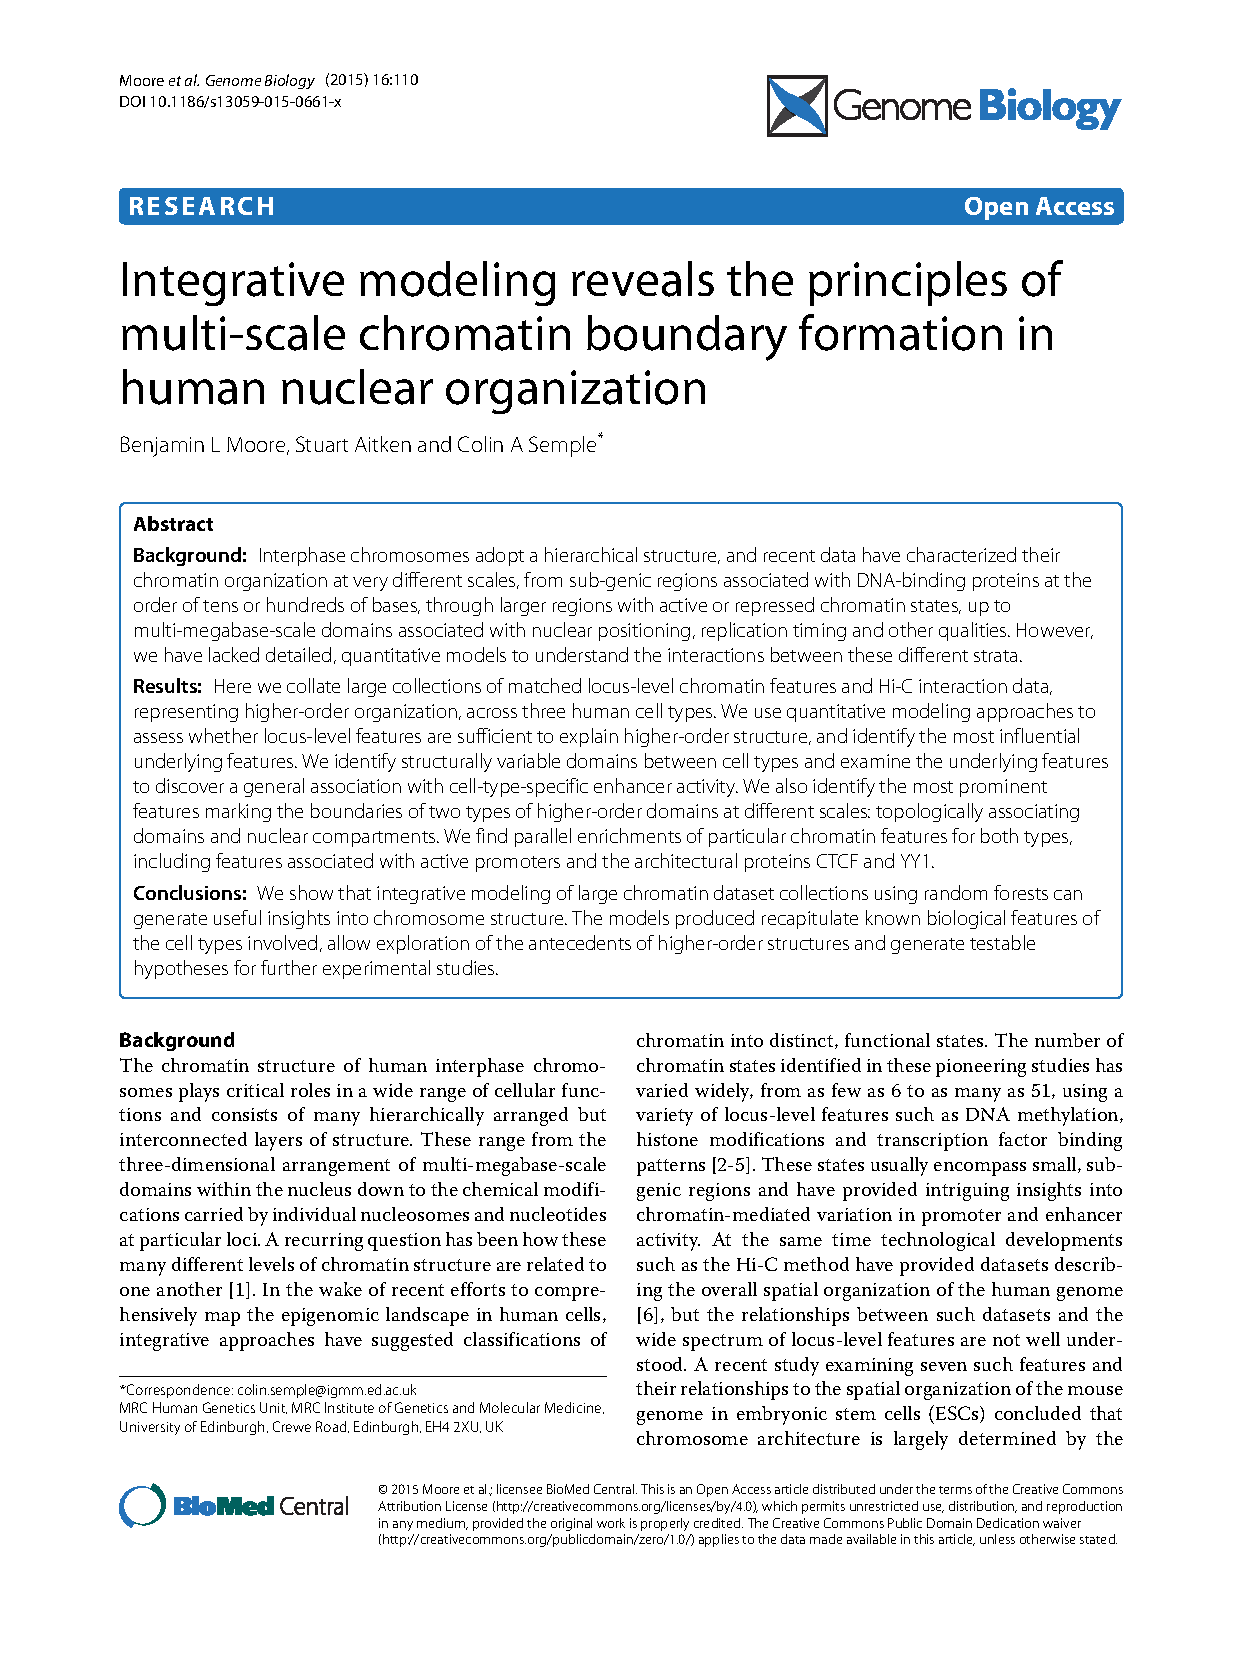
\includepdf[pages=-]{figs/genome_biol.pdf}


\ifstandalone
\begin{small}
\bibliography{/Users/benmoore/Documents/library,/Users/benmoore/Documents/customrefs}
\end{small}
\fi

\end{document}
